\section[Desenvolvimento do Projeto]{Desenvolvimento do Projeto}

Esta seção apresenta informações relativas ao desenvolvimento do projeto: localização do código-fonte e documentação, arquitetura e tecnologias utilizadas, e protótipos de tela desenvolvidos. Todas essas informações podem ser encontradas na wiki: \url{https://tools.ages.pucrs.br/plataforma-onboarding-para-novos-colaboradores/decola-wiki/-/wikis/home}.

\subsection{Repositório do Código Fonte do Projeto}
  Todo o código do projeto encontra-se distribuído em dois repositórios:
\begin{itemize}
    \item código do \textit{backend}: \url{https://tools.ages.pucrs.br/plataforma-onboarding-para-novos-colaboradores/decola-api};
    \item código do \textit{frontend}: \url{https://tools.ages.pucrs.br/plataforma-onboarding-para-novos-colaboradores/decola-frontend}.
\end{itemize}

Há, ainda, um terceiro repositório, usado somente para abrigar a wiki do projeto: \url{https://tools.ages.pucrs.br/plataforma-onboarding-para-novos-colaboradores/decola-wiki/-/wikis/home}.

\subsection{Banco de Dados Utilizado}
  O sistema de gerenciamento de banco de dados escolhido foi o PostgreSQL, um banco de dados relacional de código aberto reconhecido por sua robustez, desempenho e extensibilidade, que assegurava as propriedades \ac{acid} nas transações e a integridade referencial entre as tabelas por meio de chaves primárias e estrangeiras. O acesso aos dados foi intermediado pelo TypeORM, um \ac{orm} adotado em uma abordagem \textit{code-first}: cada entidade era declarada como uma classe anotada por \textit{decorators}, a evolução do esquema era versionada por \textit{migrations} e o acesso aos registros seguia o padrão \textit{repository}, que encapsulava as operações \ac{crud} e preservava a tipagem estática do TypeScript ao abstrair o \ac{sql} gerado.

  A modelagem foi normalizada para atender ao domínio de uma plataforma de aprendizado. No centro do esquema estava a entidade \textit{Account}, que representava as organizações e à qual se associavam os registros de \textit{User} em uma relação de um-para-muitos, diferenciados por tipos de conta e papéis --- como administradores e colaboradores. As contas vinculavam-se ainda às \textit{Areas}, o que permitia segmentar e personalizar o conteúdo por organização, bem como gerenciar de forma isolada seus usuários e materiais.

  O conteúdo educativo era organizado de forma hierárquica por meio de relações de um-para-muitos: um \textit{Course}, classificado por tipos e grupos, agregava diversos \textit{Modules}, e cada \textit{Module} reunia múltiplas \textit{Activities} --- que podiam assumir a forma de conteúdo de mídia ou de questionário. Nos questionários, cada \textit{Quiz} continha um conjunto de \textit{Questions} com alternativas corretas e incorretas, viabilizando a avaliação automática das respostas. O progresso de cada colaborador era materializado por associações que registravam os cursos, módulos e atividades concluídos, dando suporte ao acompanhamento de desempenho.

  A Figura~\ref{fig:decola-mr} apresenta o modelo relacional do banco de dados, evidenciando as principais entidades --- como \textit{Account}, \textit{User}, \textit{Area}, \textit{Course}, \textit{Module}, \textit{Activity}, \textit{Quiz} e \textit{Question} --- e os relacionamentos entre elas. A modelagem completa do banco de dados está disponível na wiki do projeto: \url{https://tools.ages.pucrs.br/plataforma-onboarding-para-novos-colaboradores/decola-wiki/-/wikis/database}.

\begin{figure}[H]
    \centering
    \small
    \caption{Modelo relacional do banco de dados}
    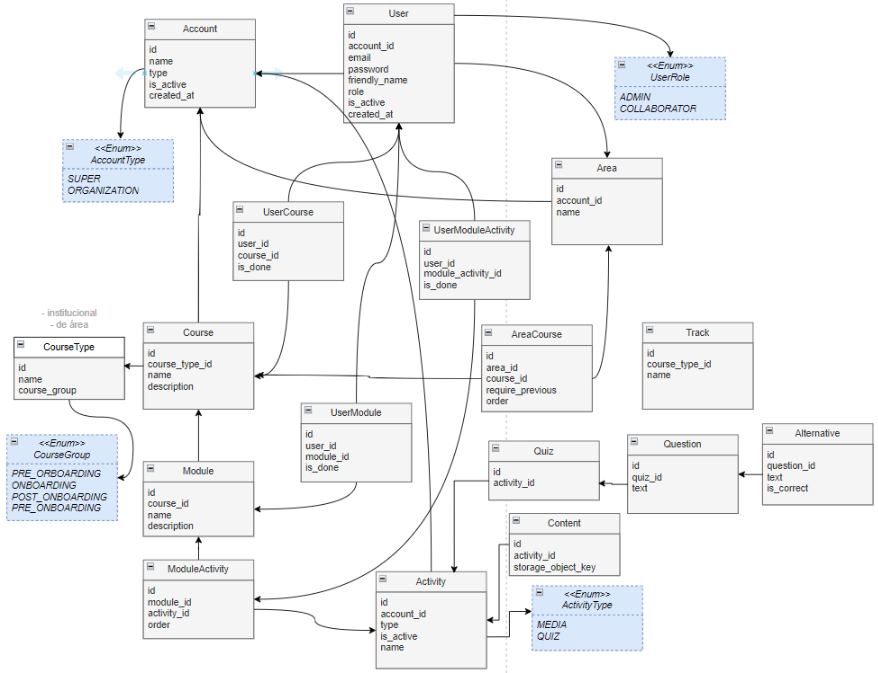
\includegraphics[width=0.9\linewidth]{conteudo/3 - ages II/images/fig4-modelo-relacional.png}

    Fonte: Wiki do projeto
    \label{fig:decola-mr}
\end{figure}

\subsection{Arquitetura Utilizada}

\subsubsection{Backend}
  O \textit{backend} do projeto foi construído como uma \ac{api} \ac{rest} utilizando o NestJS, uma estrutura para criar aplicativos Node.js eficientes e escaláveis do lado do servidor.

  Utilizamos \ac{jwt} para autenticação e autorização. O \ac{jwt} é um padrão aberto (RFC 7519) para transmitir informações seguras e confiáveis entre partes. Ele consiste em uma cadeia compacta e auto-assinada de informações codificadas em formato \ac{json}, que podem ser usadas para autenticação de usuários em aplicativos web e \textit{mobile}, bem como para comunicação entre sistemas. O fluxo de autenticação entre cliente e servidor é ilustrado na Figura~\ref{fig:decola-auth}.

\begin{figure}[H]
    \centering
    \small
    \caption{Modelo de autenticação}
    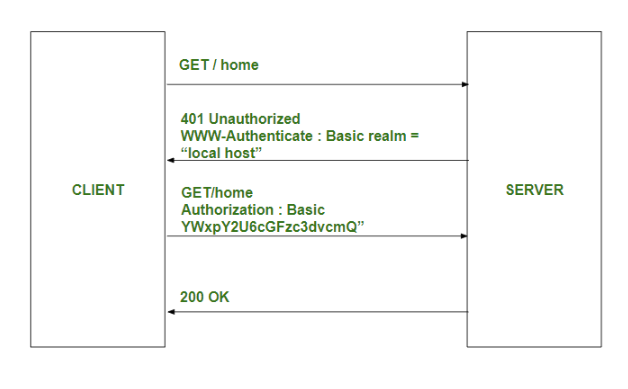
\includegraphics[width=0.9\linewidth]{conteudo/3 - ages II/images/fig5-modelo-autenticacao.png}

    Fonte: Wiki do projeto
    \label{fig:decola-auth}
\end{figure}

  O fluxo de trabalho do \ac{jwt} é dividido em três etapas:
\begin{itemize}
    \item \textbf{Geração do Token:} a primeira etapa é a geração do token \ac{jwt}. Um servidor ou aplicativo gera um token \ac{jwt} contendo as informações necessárias para autenticar o usuário. O token é geralmente gerado após o usuário fornecer suas credenciais (como nome de usuário e senha) e o servidor verificar essas credenciais. O token é assinado com uma chave secreta conhecida apenas pelo servidor ou aplicativo que o gerou.
    \item \textbf{Envio do Token:} a segunda etapa é o envio do token \ac{jwt}. O servidor ou aplicativo envia o token \ac{jwt} para o cliente, geralmente em um cabeçalho \ac{http} \texttt{Authorization}. O cliente armazena o token para uso posterior, como em solicitações subsequentes para o servidor.
    \item \textbf{Verificação do Token:} a terceira etapa é a verificação do token \ac{jwt}. O servidor ou aplicativo verifica se o token \ac{jwt} enviado pelo cliente é válido. A verificação da assinatura do token é feita usando a chave secreta. Se a assinatura estiver correta, o servidor extrai as informações do token e verifica se o usuário tem permissão para acessar o recurso solicitado. Se o token for inválido ou expirado, o servidor nega o acesso ao recurso solicitado.
\end{itemize}

\subsubsection{Frontend}
  A arquitetura de \textit{frontend} foi estruturada aplicando os conceitos de \ac{ddd} e \ac{soc}. Com \ac{ddd}, agrupamos funcionalidades com comportamentos similares e desacoplamos esses grupos ao máximo de outros componentes. Com \ac{soc}, nosso objetivo era separar lógica, \textit{views} e modelos de dados, seguindo um padrão semelhante ao \ac{mvc}.

\subsection{Protótipos das Telas Desenvolvidas}
  Os protótipos deste projeto estão disponíveis na Wiki do projeto: \url{https://tools.ages.pucrs.br/plataforma-onboarding-para-novos-colaboradores/decola-wiki/-/wikis/mockups}.

  O \textit{design} da aplicação, como pode ser visto a seguir, poderia ser aprimorado, porém à época era considerado agradável, algo que os \textit{stakeholders} aprovaram bastante. As Figuras \ref{fig:decola-tela-pagina-inicial}, \ref{fig:decola-tela-administracao} e \ref{fig:decola-tela-areas} tangem o fluxo do RH, contemplando a página inicial, a administração de colaboradores e contas, e a gestão das áreas e dos níveis de acesso. Já as Figuras \ref{fig:decola-tela-multipla-escolha} e \ref{fig:decola-tela-conteudo-externo} abrangem o fluxo do colaborador, apresentando uma atividade de múltipla escolha e uma atividade de conteúdo externo tal como elas são exibidas ao usuário durante a realização de um módulo.

\begin{figure}[H]
    \centering
    \small
    \caption{Tela de página inicial}
    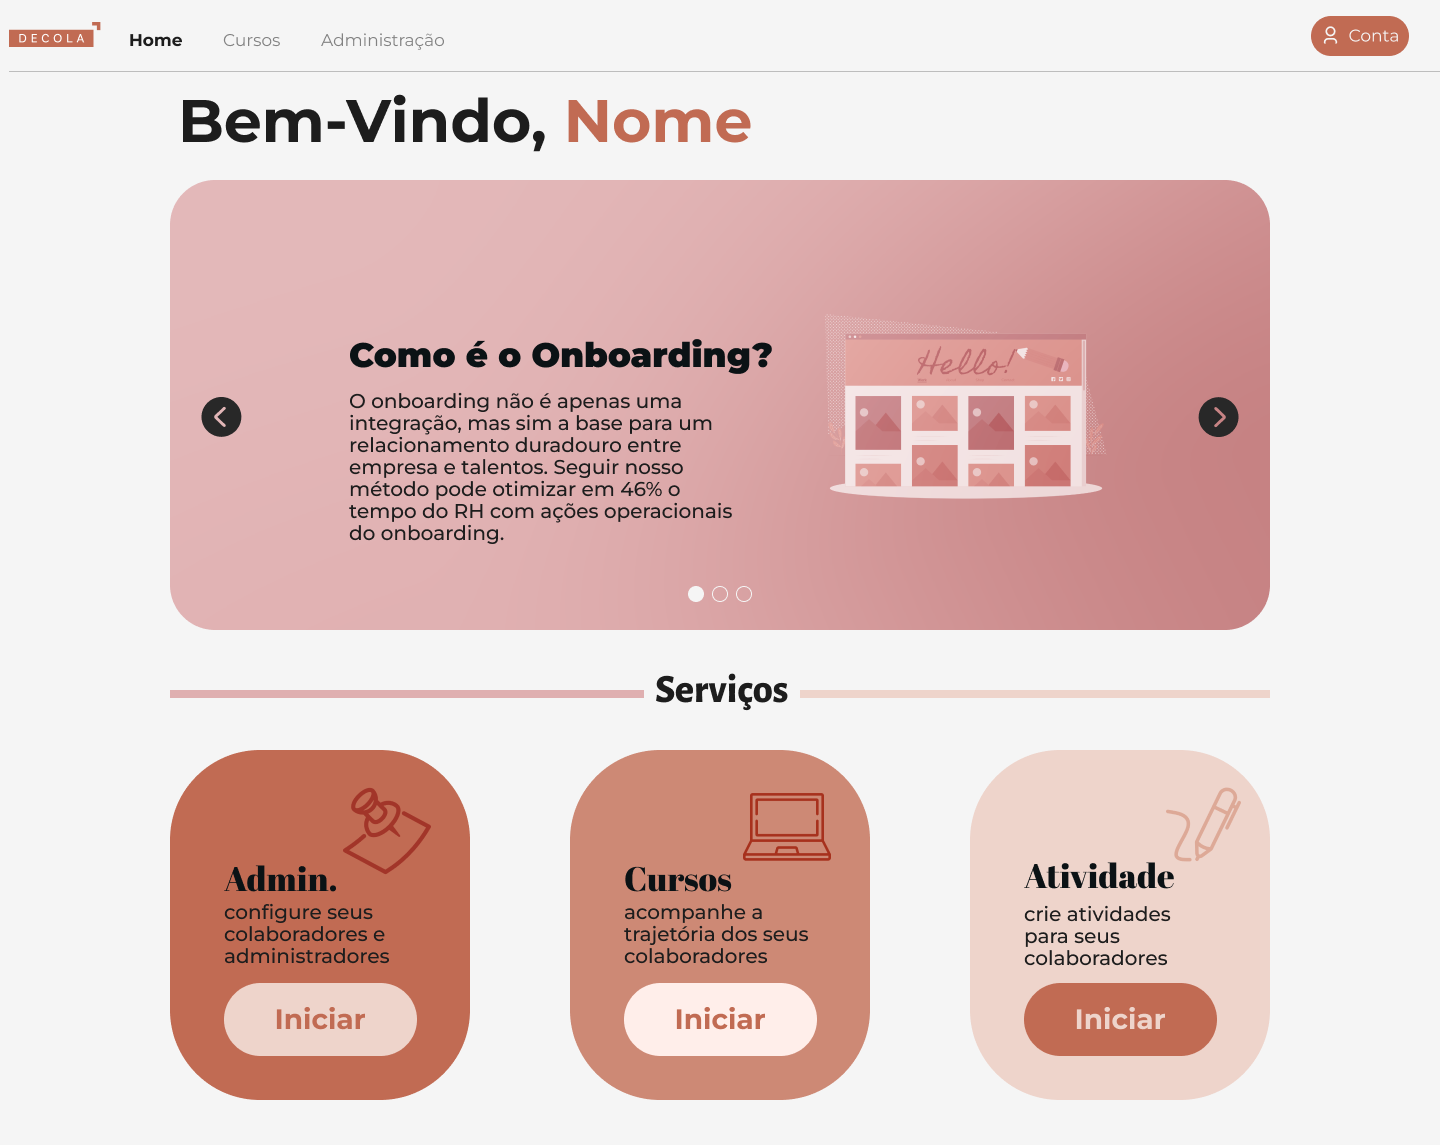
\includegraphics[width=0.8\linewidth,height=0.34\textheight,keepaspectratio]{conteudo/3 - ages II/images/fig5a-tela-pagina-inicial.png}

    Fonte: Wiki do projeto
    \label{fig:decola-tela-pagina-inicial}
\end{figure}

\begin{figure}[H]
    \centering
    \small
    \caption{Tela de administração}
    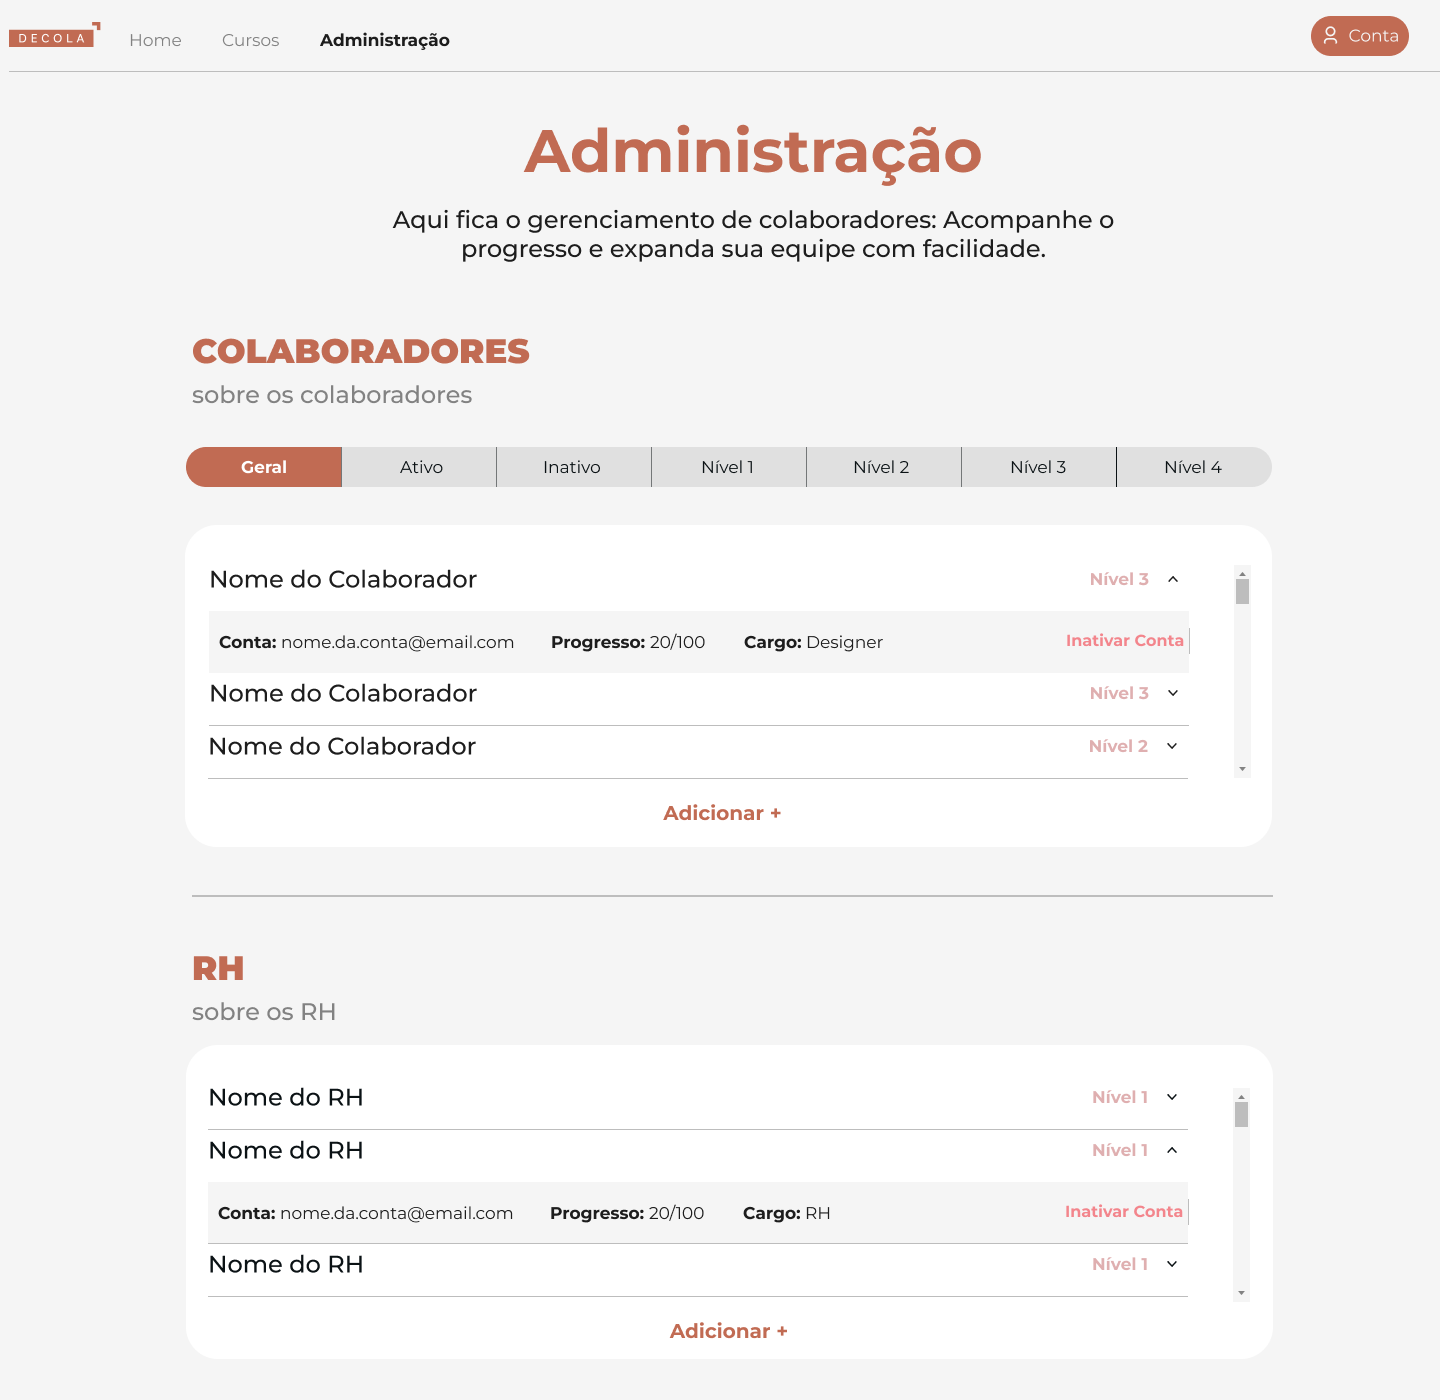
\includegraphics[width=0.8\linewidth,height=0.34\textheight,keepaspectratio]{conteudo/3 - ages II/images/fig5b-tela-administracao.png}

    Fonte: Wiki do projeto
    \label{fig:decola-tela-administracao}
\end{figure}

\begin{figure}[H]
    \centering
    \small
    \caption{Tela de áreas}
    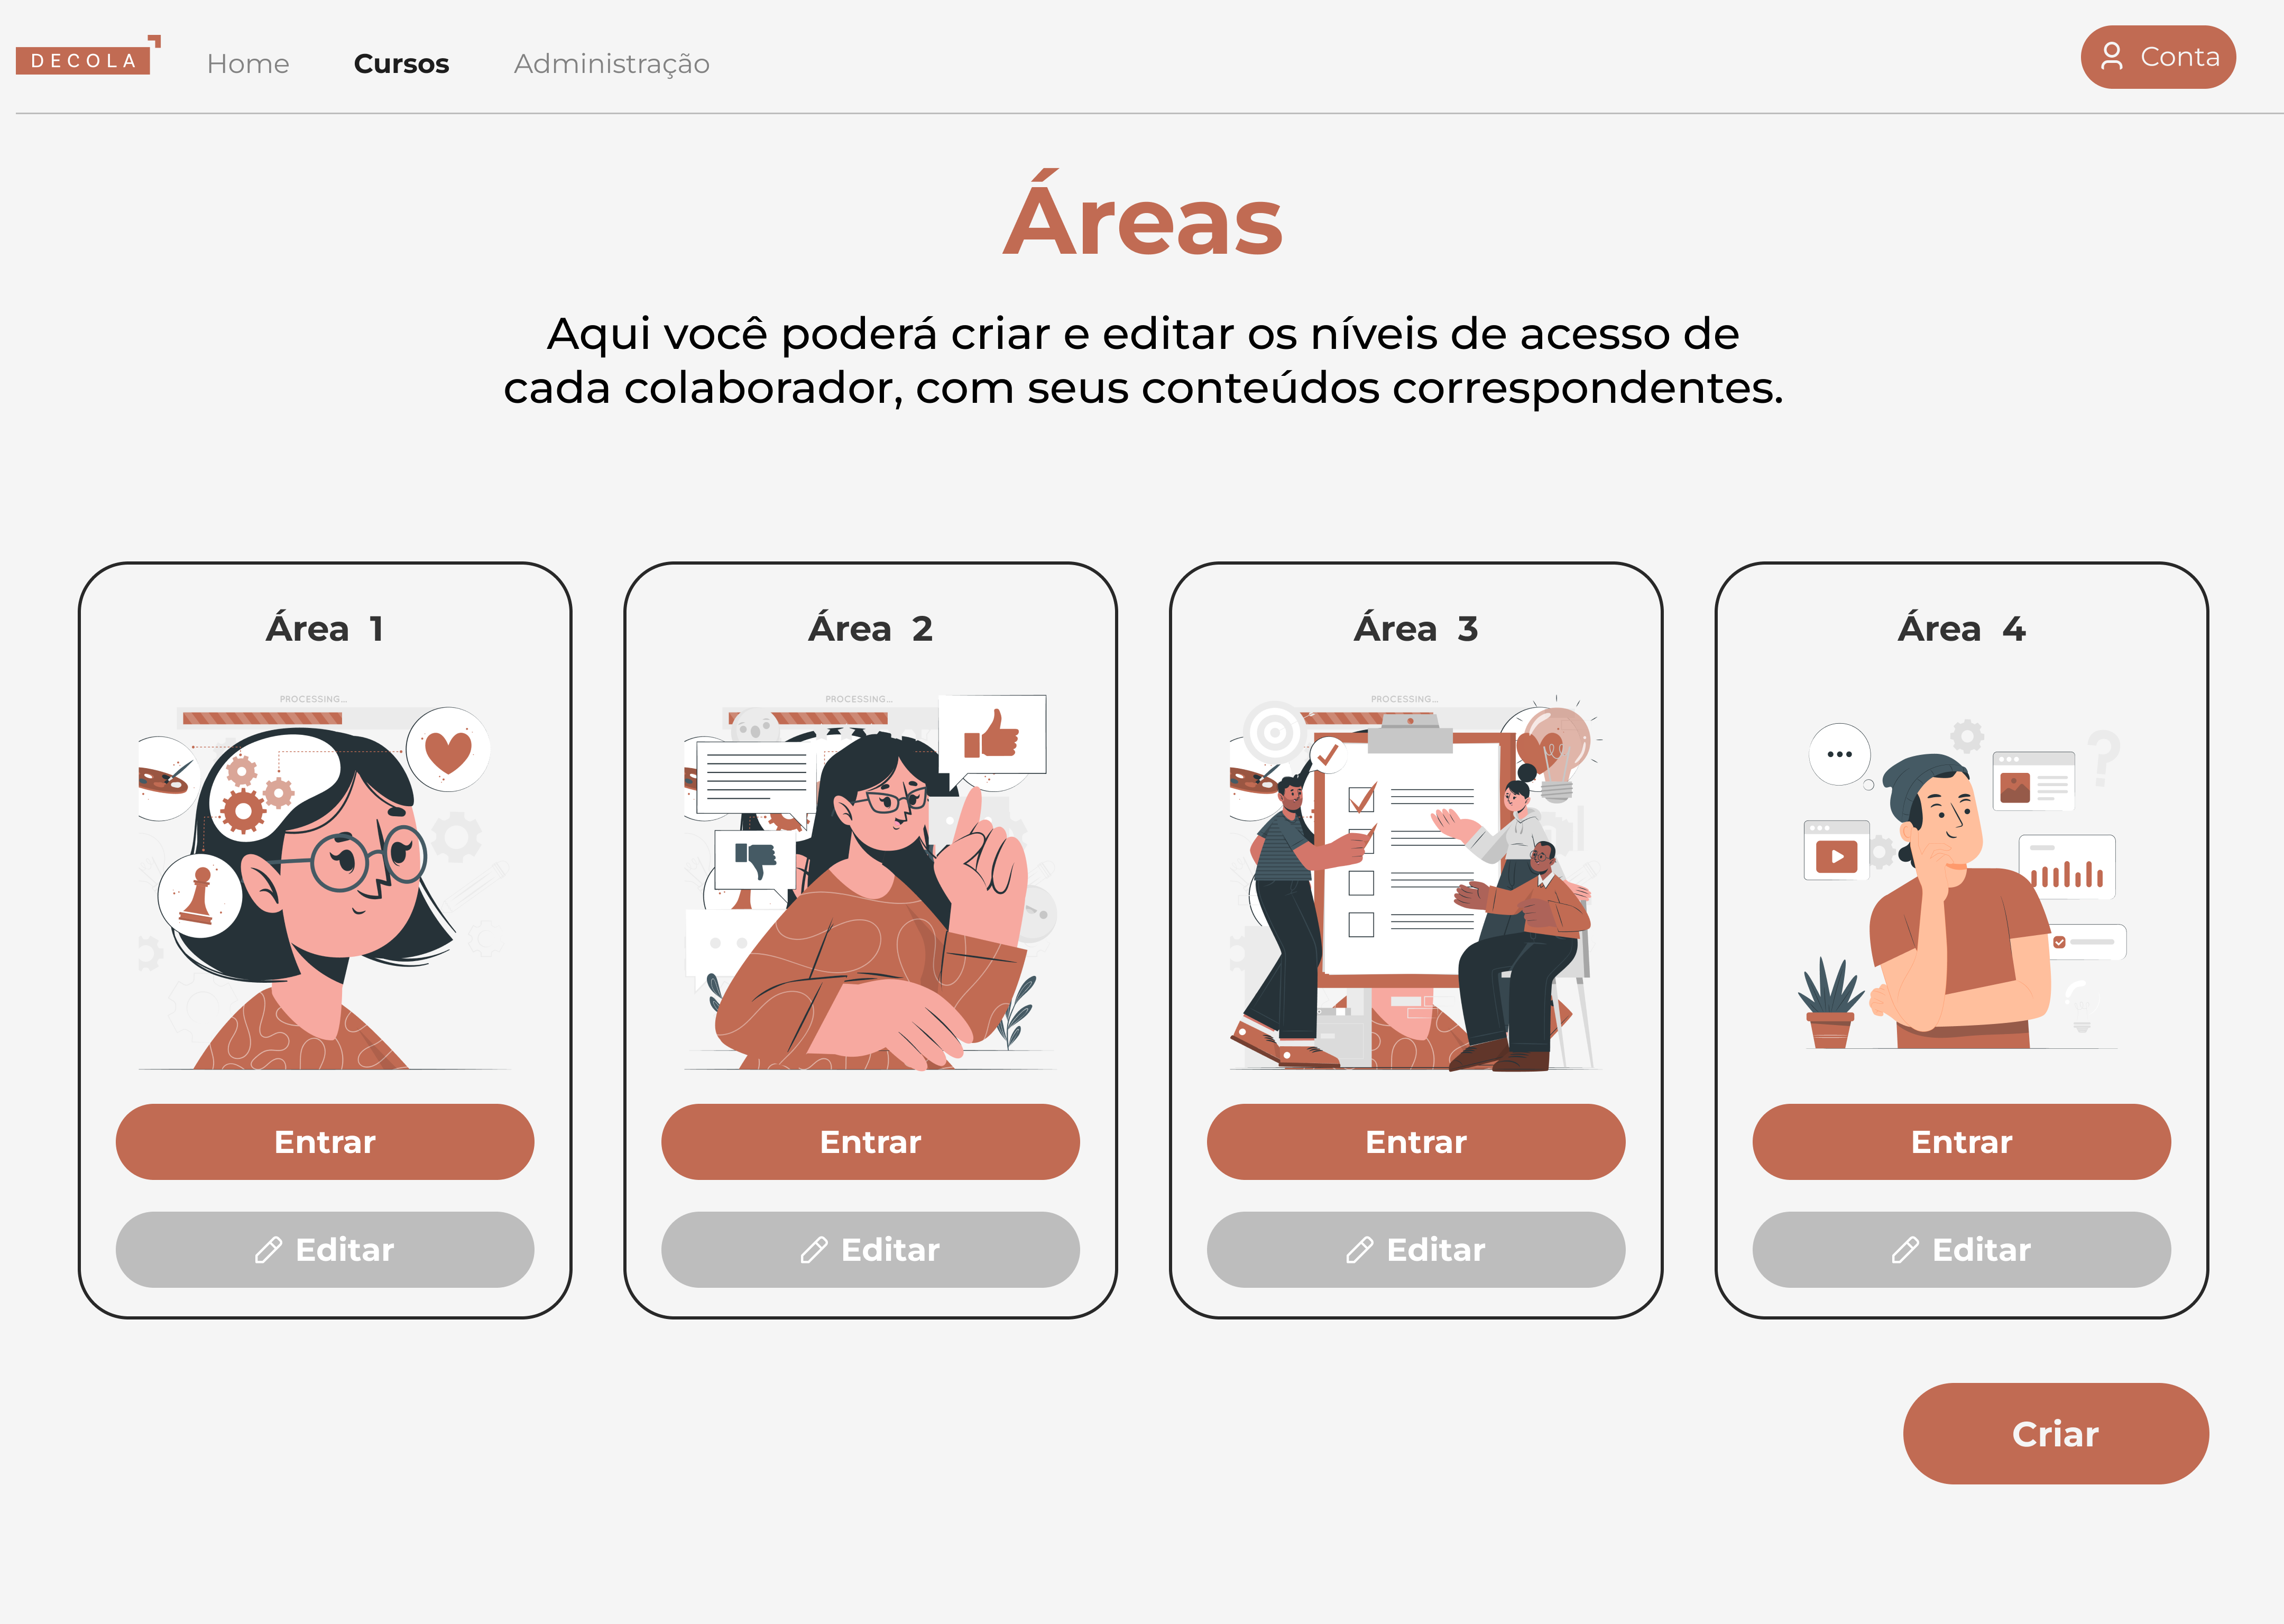
\includegraphics[width=0.9\linewidth,height=0.34\textheight,keepaspectratio]{conteudo/3 - ages II/images/fig5c-tela-areas.png}

    Fonte: Wiki do projeto
    \label{fig:decola-tela-areas}
\end{figure}

\begin{figure}[H]
    \centering
    \small
    \caption{Tela de atividade de múltipla escolha}
    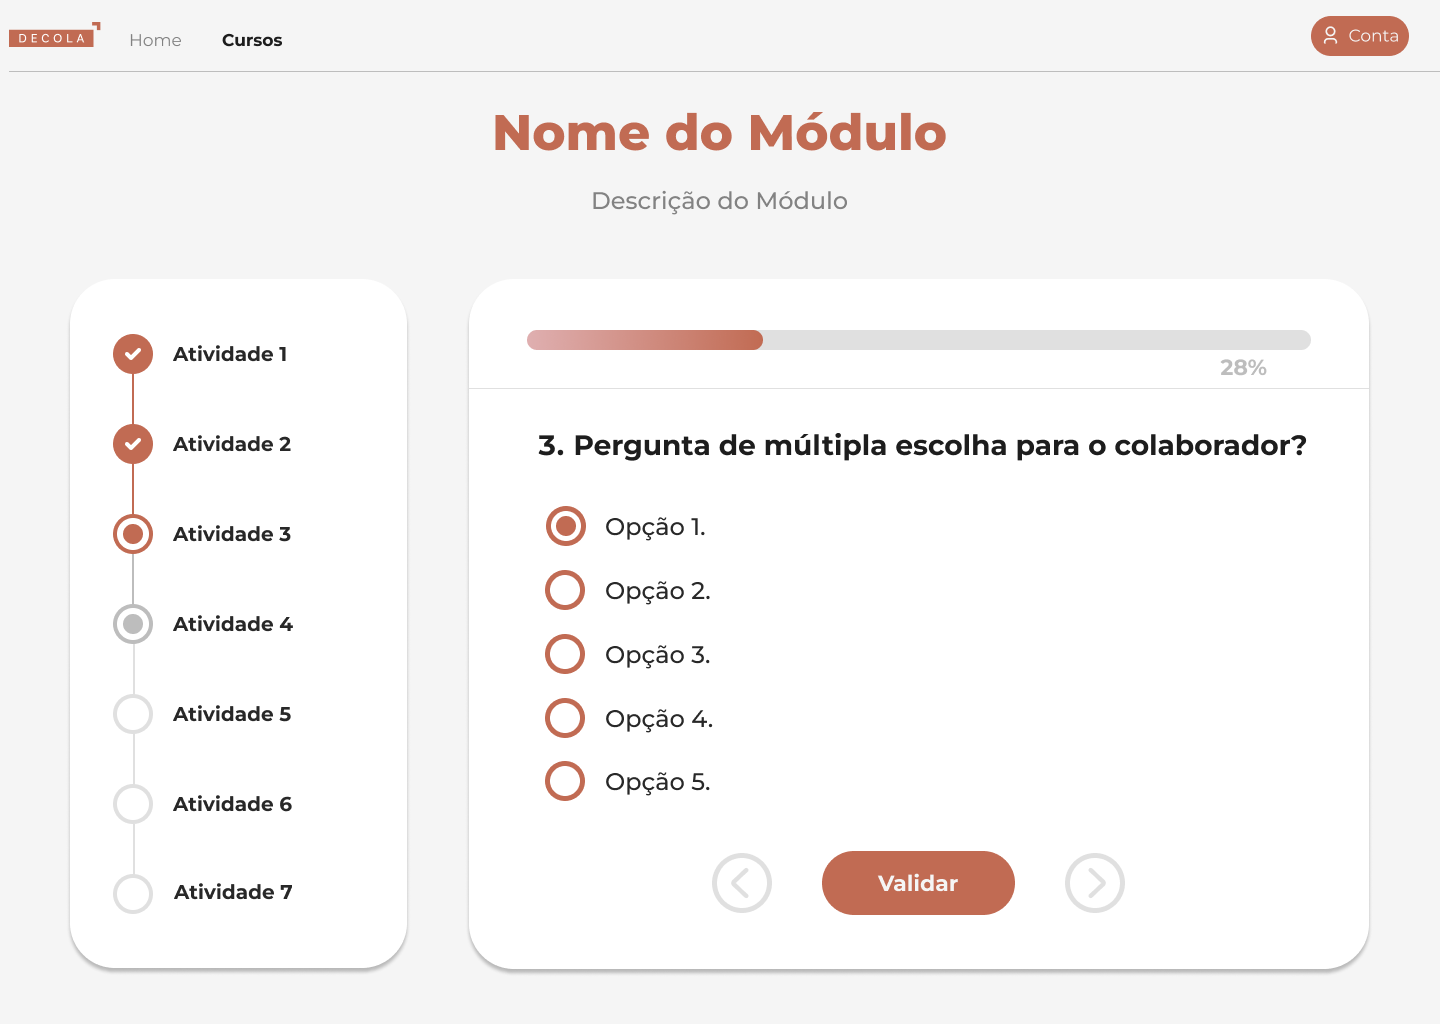
\includegraphics[width=0.8\linewidth,height=0.34\textheight,keepaspectratio]{conteudo/3 - ages II/images/fig5d-tela-multipla-escolha.png}

    Fonte: Wiki do projeto
    \label{fig:decola-tela-multipla-escolha}
\end{figure}

\begin{figure}[H]
    \centering
    \small
    \caption{Tela de atividade de conteúdo externo}
    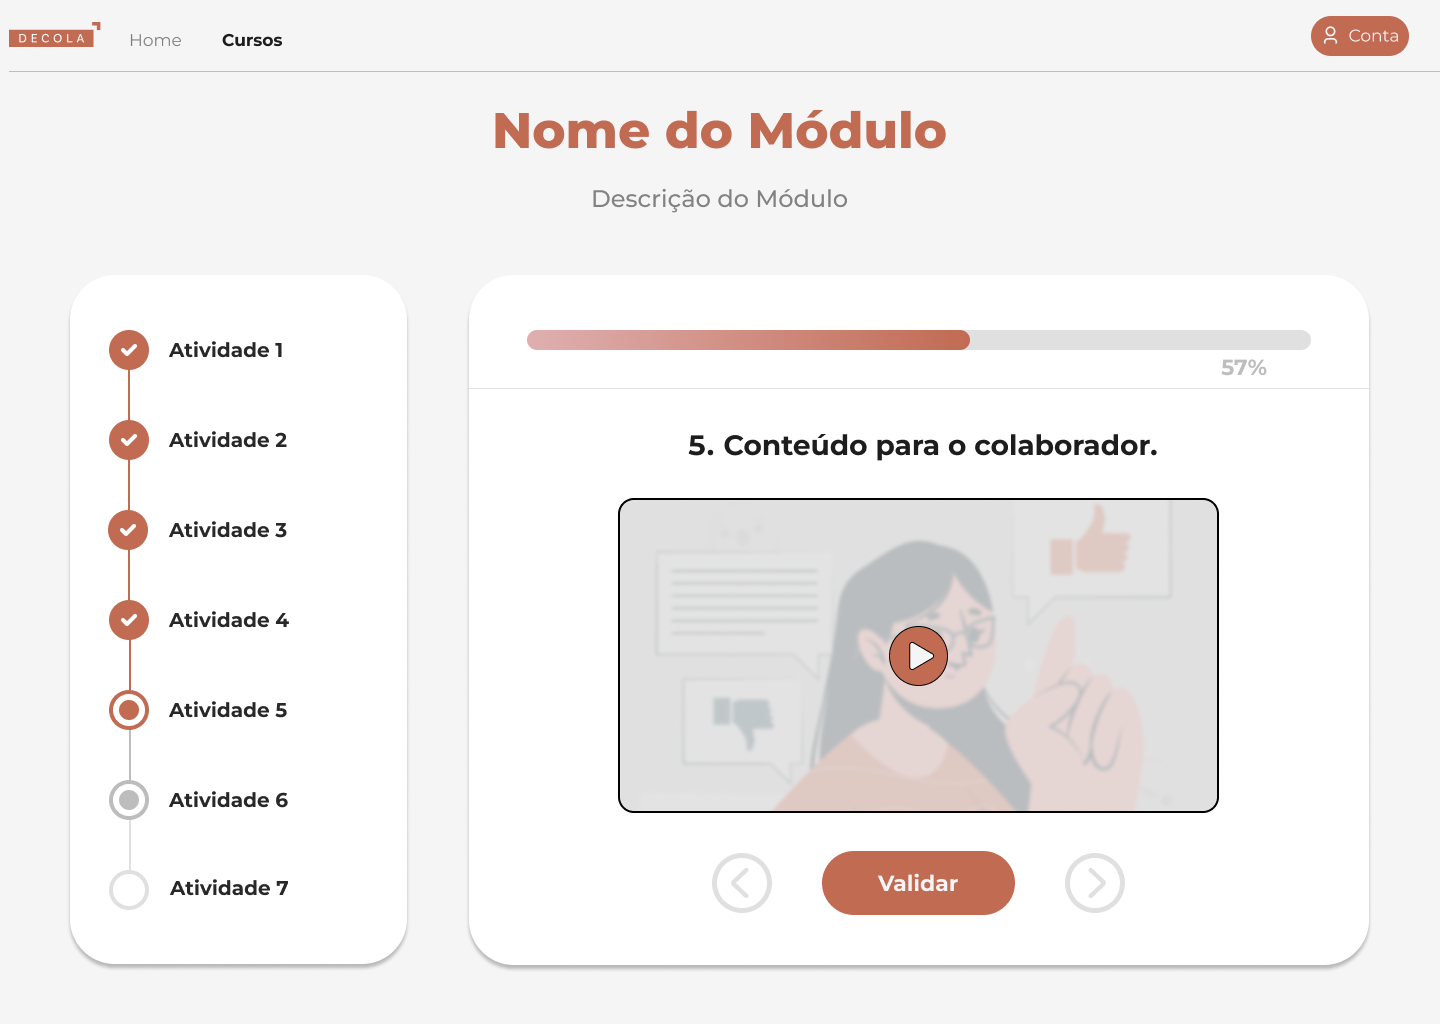
\includegraphics[width=0.8\linewidth,height=0.34\textheight,keepaspectratio]{conteudo/3 - ages II/images/fig5e-tela-conteudo-externo.png}

    Fonte: Wiki do projeto
    \label{fig:decola-tela-conteudo-externo}
\end{figure}

\subsection{Tecnologias Utilizadas}

\begin{itemize}
    \item \textbf{PostgreSQL} \parencite{postgresql}: Sistema de gerenciamento de banco de dados relacional de código aberto, conhecido por sua robustez, extensibilidade e conformidade com os padrões \ac{sql}.
    \item \textbf{TypeORM} \parencite{typeorm}: Biblioteca \ac{orm} para TypeScript e JavaScript que facilita a interação com bancos de dados relacionais por meio de um mapeamento objeto-relacional eficiente e intuitivo.
    \item \textbf{AWS} \parencite{aws}: Plataforma de computação em nuvem fornecida pela Amazon, oferecendo uma ampla gama de serviços, incluindo armazenamento, redes, bancos de dados e ferramentas de desenvolvimento, para escalabilidade e flexibilidade na construção de aplicações.
    \item \textbf{TypeScript} \parencite{typescript}: Linguagem de programação de código aberto desenvolvida pela Microsoft que adiciona tipagem estática opcional ao JavaScript, melhorando a produtividade e a qualidade do código.
    \item \textbf{NestJS} \parencite{nestjs}: \textit{Framework} progressivo para Node.js que permite a construção de aplicativos do lado do servidor escaláveis e eficientes utilizando TypeScript.
    \item \textbf{React} \parencite{react}: Biblioteca JavaScript de código aberto para a construção de interfaces de usuário, desenvolvida pelo Facebook, amplamente utilizada para criar aplicações web e \textit{mobile} dinâmicas e interativas.
    \item \textbf{Sass} \parencite{sass}: Extensão do CSS que permite o uso de variáveis, aninhamento e \textit{mixins}, facilitando a escrita e manutenção de estilos, tornando o desenvolvimento \textit{front-end} mais eficiente.
\end{itemize}
